\documentclass[14pt]{beamer}
\usepackage[T2A]{fontenc}
\usepackage[utf8]{inputenc}
\usepackage[english]{babel}
\usepackage{amssymb,amsfonts,amsmath,mathtext}
\usepackage{cite,enumerate,float,indentfirst}

\usepackage{multicol}
\usepackage{listings}


\usetheme{Pittsburgh}
\usecolortheme{whale}

\setlength{\columnseprule}{1pt}
\def\columnseprulecolor{\color{blue}}

\setbeamercolor{footline}{fg=blue}
\setbeamertemplate{footline}{
  \leavevmode%
  \hbox{%
  \begin{beamercolorbox}[wd=.333333\paperwidth,ht=2.25ex,dp=1ex,center]{}%
    Boris Kudryashov, ITMO University
  \end{beamercolorbox}%
  \begin{beamercolorbox}[wd=.333333\paperwidth,ht=2.25ex,dp=1ex,center]{}%
    St. Petersburg, 2016
  \end{beamercolorbox}%
  \begin{beamercolorbox}[wd=.333333\paperwidth,ht=2.25ex,dp=1ex,right]{}%
  Page \insertframenumber{} of \inserttotalframenumber \hspace*{2ex}
  \end{beamercolorbox}}%
  \vskip0pt%
}

\newcommand{\itemi}{\item[\checkmark]}

\title{\small{Information Theory. 5th Chapter Problems}}
\author{\huge{
Boris Kudryashov \\
\vspace{30pt}
ITMO University
}}


\begin{document}

\maketitle

  

\begin{frame}
\frametitle{Problems}
\begin{enumerate}
% \footnotesize {
  
    \begin{figure}[ht]
    \begin{minipage}{1.0\linewidth}
    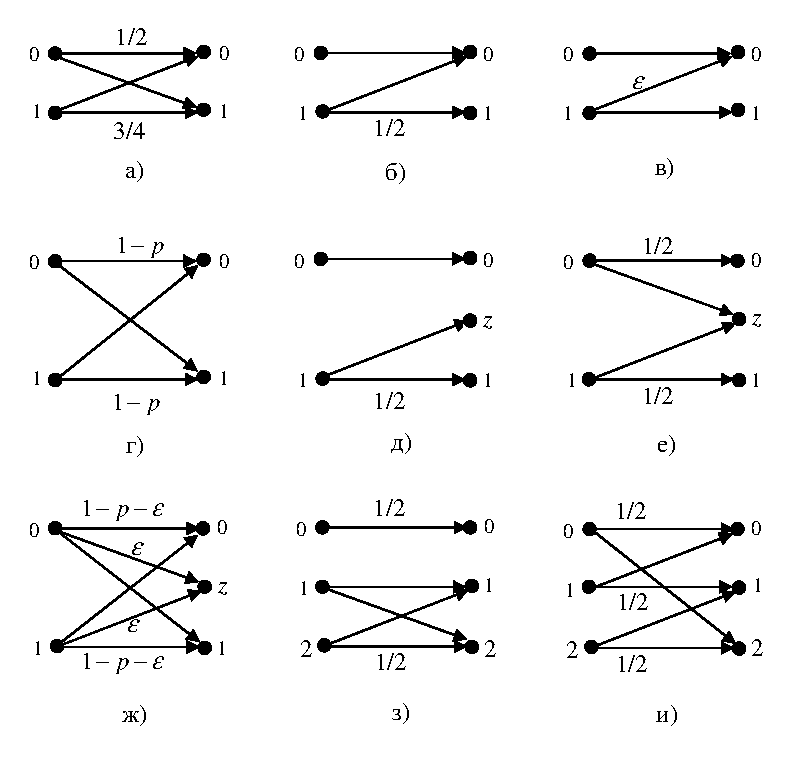
\includegraphics[width=0.85\textwidth]{chann_ex.eps}
    %\centerline{\includegraphics[width=3.16in,height=4.02in]
    \label{chan_ex}
    \end{minipage}
    \end{figure}
    
\end{enumerate}
\end{frame}    
    
\begin{frame}
\frametitle{Problems}
\begin{enumerate}
    \item[1]
    For the channel at pic.\ref{chan_ex}a, with a uniform input alphabet $X$, calculate the mutual information $I\left( {x;y} \right),x \in X,y \in Y$ and the average mutual information $I\left( {X;Y} \right)$. Explain the results.
    
\end{enumerate}
\end{frame}    
    
\begin{frame}
\frametitle{Problems}
\begin{enumerate}    
    
    \item[2]
    For the channel at pic.\ref{chan_ex}б, draw a plot of dependence between $I\left( {X;Y} \right)$ and  $p\left( {x = 1}
    \right) = p$ without doing calculations and without using properties of mutual information.
 
\end{enumerate}
\end{frame}    
    
\begin{frame}
\frametitle{Problems}
\begin{enumerate} 
    
    \item[3]
    For the channel at pic.\ref{chan_ex}в, draw a plot mutual information as a functions of $\varepsilon $, assuming uniform alphabet, without doing calculations and without using properties of mutual information.

\end{enumerate}
\end{frame}    
    
\begin{frame}
\frametitle{Problems}
\begin{enumerate}
    
    \item[4]
    For channels at pic.\ref{chan_ex}г-\ref{chan_ex}и, calculate the channel throughput.

\end{enumerate}
\end{frame}

\end{document} 